\section{Results}

\subsection{Network Benchmarks}

\begin{figure}
	\centering
	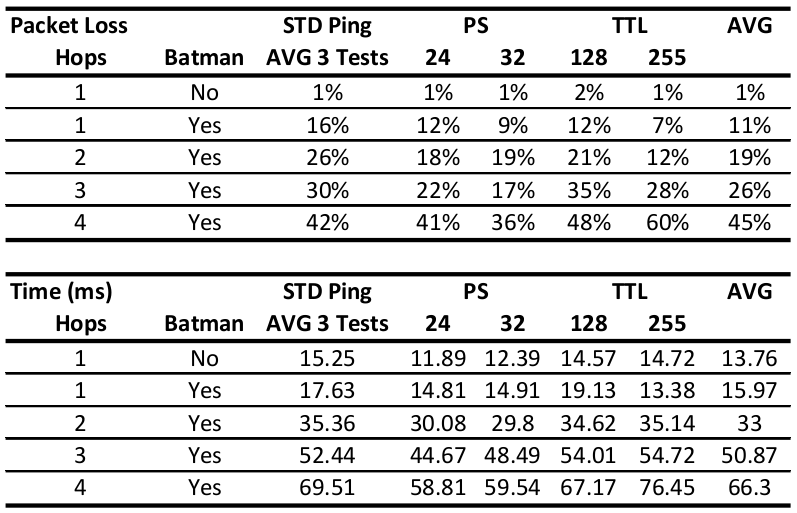
\includegraphics[scale=0.3]{902sheet}
	\caption{The data received from operating at 902/915 MHz.}
	\label{fig:902}
\end{figure}

\begin{figure}
	\centering
	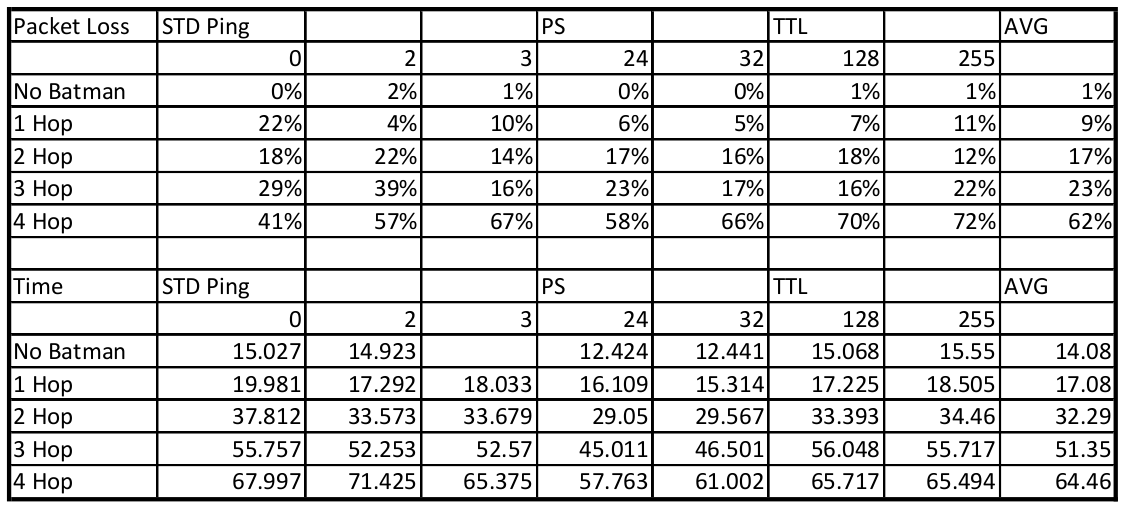
\includegraphics[scale=0.3]{2400}
	\caption{The data received from operating at 2.4/2.5 GHz.}
	\label{fig:2400}
\end{figure}

\begin{figure}
	\centering
	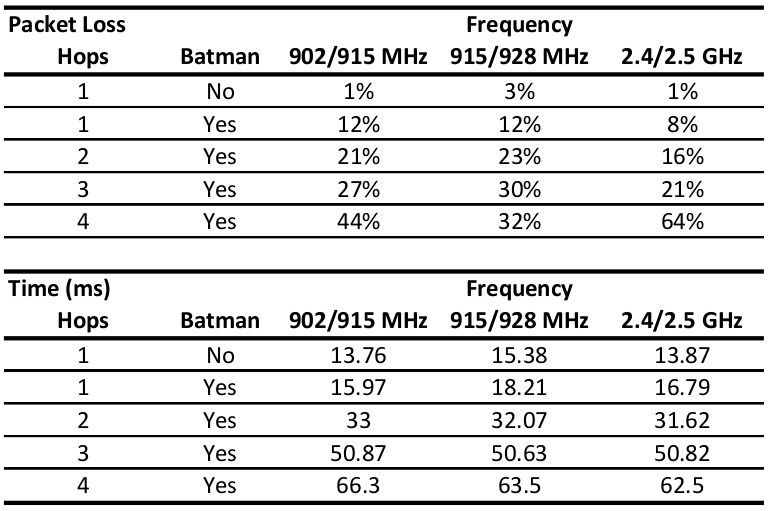
\includegraphics[scale=0.3]{alldata}
	\caption{The Averages from all three tests.}
	\label{fig:alldata}
\end{figure}

The results of the Network Benchmark tests from section 4 part A are summarized in Figure \ref{fig:alldata}. In all cases, the single point to point communication, without the Batman-adv protocol running, resulted in a much lower packet loss. This served as our control group. However,in the two sets of lower frequency ratings, the packet loss remained below 50\%. Also, the increase in time as hops were added has a roughly linear change. This means the overhead of adding more hops is not unmanageable. A full listing of tests run for the 902/915 MHz, and 2.4/2.5 GHz cases are provided in Figure \ref{fig:902} and Figure \ref{fig:2400} respectively. These tables show that running at the higher frequencies causes the SDRN to drop a lot more packets, especially when moving through the full four hops.  


\subsection{Route Changes}

\begin{figure*}
	\centering
	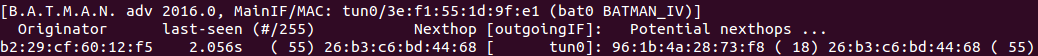
\includegraphics[scale=0.5]{2PotentialHops}
	\caption{The initial condition, where there are two possible routes the packet can take.}
	\label{fig:2Hops}
\end{figure*}

\begin{figure*}
	\centering
	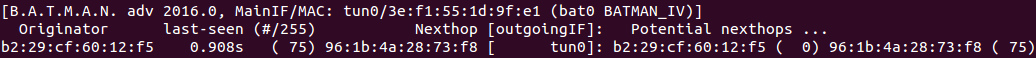
\includegraphics[scale=0.5]{hopchange}
	\caption{After the gain is reduced, the packets are now routing through a different node.}
	\label{fig:NewHop}
\end{figure*}

The route changing feature of Batman-adv showed success with our test setup from section 4 part B. Initially, batctl reported two possible links. One with a link quality of 55, and the other with a link quality of 18. As we decreased the gain of the intermediate node, the link quality reported by batctl also decreased. Eventually, Batman-adv switched and began using the other node. At this point it no longer saw the original node, and reported a link quality of 75 on the alternate one. The initial setup can be seen in Figure \ref{fig:2Hops}. After the change, the routing table appeared as it does in Figure \ref{fig:NewHop}. This feature works in the SDR system, and can continue to be used without significant changes.  

\subsection{Frequency Changes}

Using A.L.F.R.E.D. to distribute frequency hopping showed mixed results. Using the setup from section 4 part C, we were able to get the Nodes to change frequency in unison, but not reliably. A.L.F.R.E.D. itself is designed for a traditional Wi-Fi environment, and therefore does not have an expectation that the other nodes will become completely unreachable due to changes in operating frequency \cite{0015}. We were finding that some nodes would switch before A.L.F.R.E.D. had propagated the data table to the other nodes. This would leave one node with an out-of-date table, meaning it would not make the frequency change. In the current iteration of the project, there is no way for these orphaned nodes to find the rest of the network again. Figure \ref{fig:freqshift} shows a situation in which four out of five nodes were able to make the jump, with one node remaining at the original frequency.



